\documentclass[11pt]{article}
\usepackage[utf8]{inputenc}
\usepackage{amsfonts}
\usepackage{natbib}
\usepackage{graphicx}
\usepackage{amsmath}
\usepackage{amssymb}
\usepackage{mathrsfs} % Cursive font
\usepackage{graphicx}
\usepackage{ragged2e}
\usepackage{fancyhdr}
\usepackage{nameref}
\usepackage{wrapfig}
\usepackage{listings}

% to set spacing between lines
\usepackage{setspace}

% to rotate content 90 degrees
\usepackage{lscape}



% defining command for the curly arrow
\newcommand{\curly}{\mathrel{\leadsto}}


\usepackage{mathtools}
\usepackage{xparse} \DeclarePairedDelimiterX{\Iintv}[1]{\llbracket}{\rrbracket}{\iintvargs{#1}}
\NewDocumentCommand{\iintvargs}{>{\SplitArgument{1}{,}}m}
{\iintvargsaux#1}
\NewDocumentCommand{\iintvargsaux}{mm} {#1\mkern1.5mu,\mkern1.5mu#2}

\makeatletter
\newcommand*{\currentname}{\@currentlabelname}
\makeatother

\usepackage[a4paper,hmargin=1in, vmargin=1.4in,footskip=0.25in]{geometry}


%\addtolength{\hoffset}{-1cm}
%\addtolength{\hoffset}{-2.5cm}
%\addtolength{\voffset}{-2.5cm}
\addtolength{\textwidth}{0.2cm}
%\addtolength{\textheight}{2cm}
\setlength{\parskip}{8pt}
\setlength{\parindent}{0.5cm}
\linespread{1.5}

\pagestyle{fancy}
\fancyhf{}
\rhead{TP2 - Sullivan}
\lhead{Seguridad Informática}
\rfoot{\vspace{1cm} \thepage}

\renewcommand*\contentsname{\LARGE Índice}

\begin{document}

\begin{titlepage}
    \begin{center}
        \vfill
        \vfill
            \vspace{0.7cm}
            \noindent\textbf{\Huge Trabajo Práctico 2}\par
            \noindent\textbf{\Huge Seguridad Informática}\par
            \vspace{.5cm}
        \vfill
        \noindent \textbf{\huge Alumna:}\par
        \vspace{.5cm}
        \noindent \textbf{\Large Sullivan, Katherine}\par
 
        \vfill
        \large Universidad Nacional de Rosario \par
        \noindent\large 2023
    \end{center}
\end{titlepage}
\ \par


% Setting the spacing between lines
\setstretch{0}

\section{Buffer Overflow}

\subsection{Apagando las contramedidas}
Para empezar con el ataque, debemos apagar las contramedidas que se nos indican en el laboratorio. 

\begin{center}
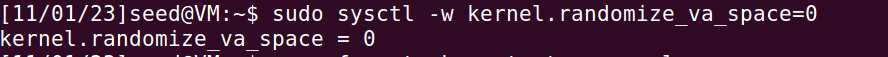
\includegraphics[scale=0.7]{deshab1.png}
\end{center}

\begin{center}
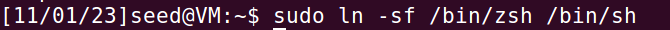
\includegraphics[scale=0.8]{deshab2.png}
\end{center}

\subsection{Corriendo el shellcode}
Para familiarizarnos con su funcionamiento el laboratorio pone como tarea el correr el shellcode, así que eso hacemos

\begin{center}
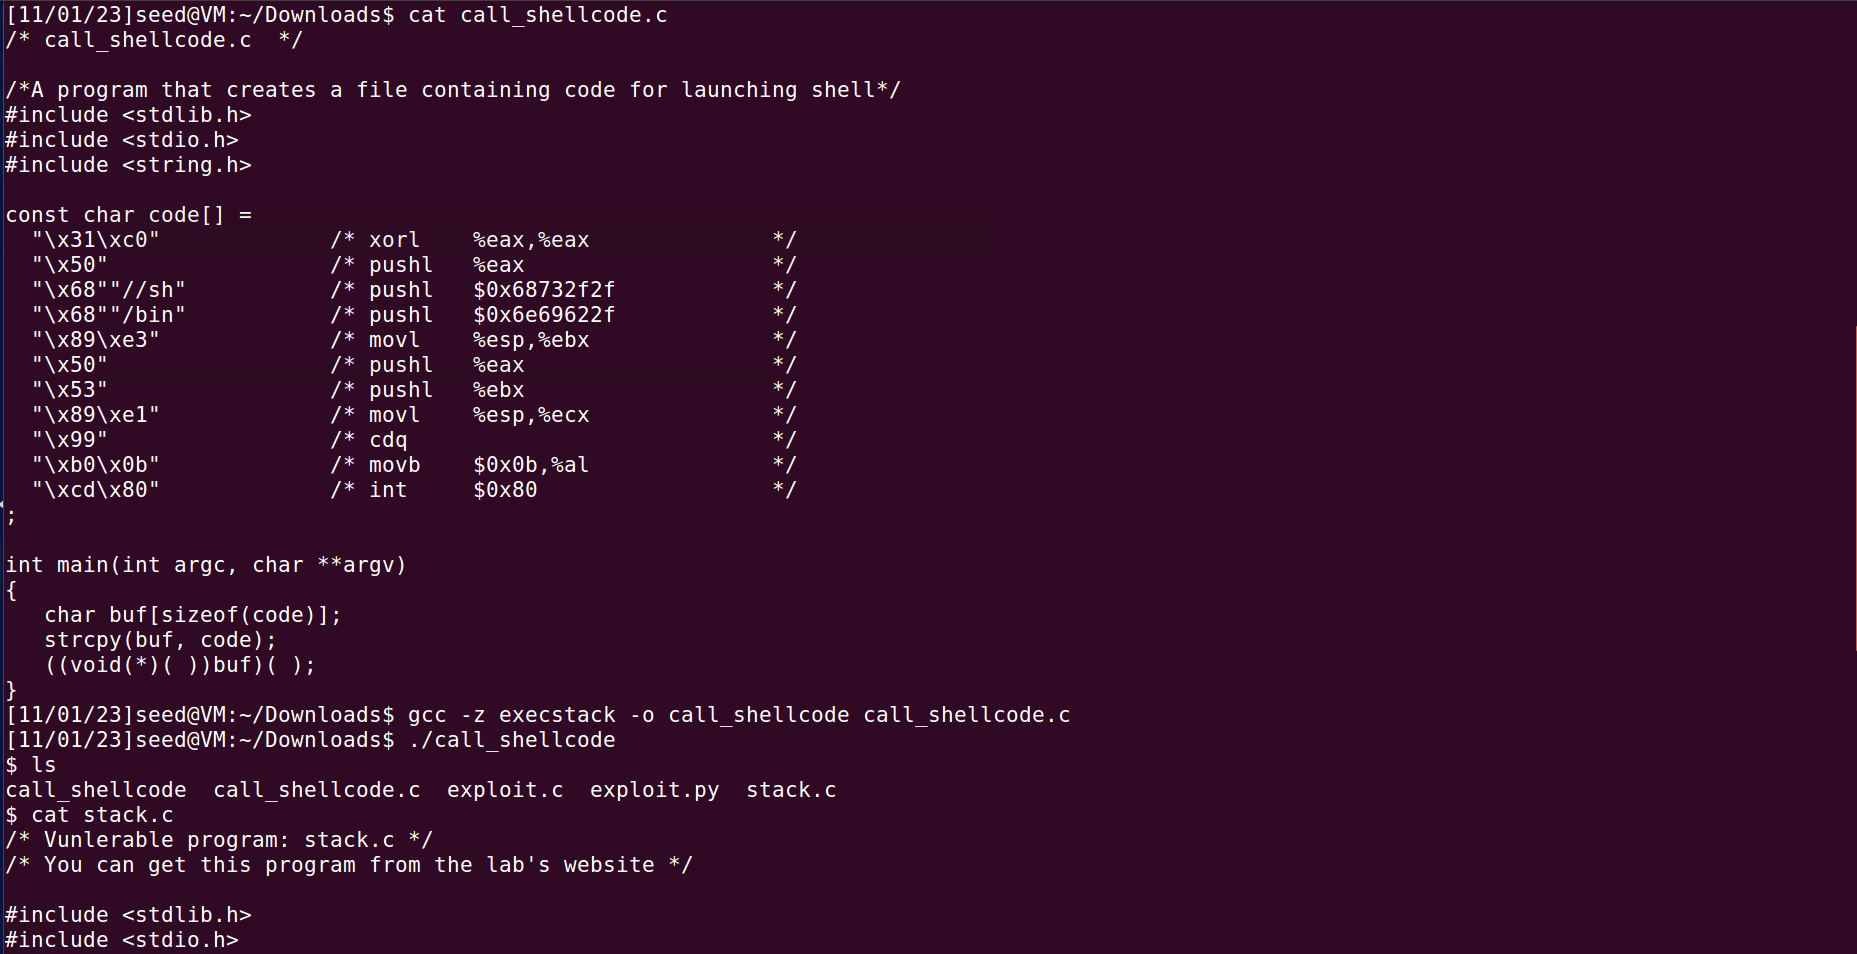
\includegraphics[scale=0.4]{call_shellcode_exec.png}
\end{center}

\subsection{Explotando la vulnerabilidad}


\newpage

\section{PCC}

\subsection*{A. Descripción del programa}

\begin{center}
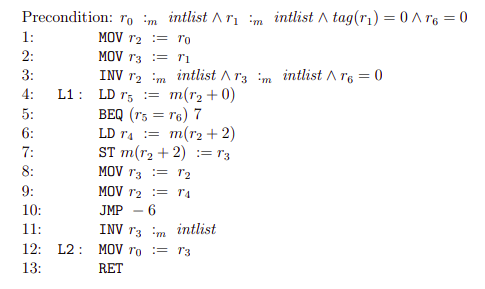
\includegraphics[scale=0.7]{progPCC.png}
\end{center}

Podemos entender el programa como un bucle entre las 
líneas L1 y L2, el cual se ejecuta hasta que la lista
en $r_2$ queda vacía.

Lo almacenado en $r_2$ comienza siendo la lista argumento $r_0$, lo almacenado en $r_3$, 
una lista vacía y el funcionamiento dentro del bucle 
es el siguiente:

En $r_4$ se guarda la \textit{tail} de la de la lista en $r_2$, mientras que 
se guarda como \textit{next} del primer elemento de la lista $r_2$
a $r_3$, y luego, se pasa esa lista armada por el \textit{head} de $r_2$ y $r_3$ a $r_3$, mientras que
lo guardado en $r_4$ (la \textit{tail}) pasa a $r_2$ y se 
repite el ciclo.

Esto, en resumen, lo que logra es que en $r_3$ se vaya
reconstruyendo lo que había en la lista $r_0$ pero de manera inversa
y esto es lo que devolverá la función. 

\textbf{El programa es una implementación de la función inverse para listas de enteros}

\subsection*{B. Computación de la condición de verificación}

\begin{flalign*}
VC_{13} = true &&\\\nonumber 
\end{flalign*}

\begin{flalign*}
VC_{12} &= VC_{13}[r_3/r_0] &&\\\nonumber 
        &= true &&\\\nonumber 
\end{flalign*}

\begin{flalign*}
VC_{11} &= r_3 :_{m} intlist &&\\\nonumber 
\end{flalign*}

\begin{flalign*}
VC_{10} &= VC_{10+(-6)-1} &&\\\nonumber 
        &= VC_{3} &&\\\nonumber 
        &= r_2 :_m intlist \wedge r_3 :_m intlist \wedge (r_6 = 0) &&\\\nonumber 
\end{flalign*}

\begin{flalign*}
VC_{9} &= VC_{10}[r_4/r_2] &&\\\nonumber 
       &=r_4 :_m intlist \wedge r_3 :_m intlist 
            \wedge (r_6 = 0) &&\\\nonumber 
\end{flalign*}

\begin{flalign*}
VC_{8} &= VC_{9}[r_2/r_3] &&\\\nonumber 
       &= r_4 :_m intlist \wedge r_2 :_m intlist 
\wedge (r_6=0) &&\\\nonumber 
\end{flalign*}


\begin{flalign*}
VC_{7} &= VC_{8}[upd(m, r_2+2, r_3)/m] \wedge writable(r_2+2) &&\\\nonumber 
   &= r_4 :_{upd(m, r_2+2, r_3)} intlist
\wedge r_2 :_{upd(m, r_2+2, r_3)} intlist 
\wedge (r_6=0) \wedge writable(r_2+2) &&\\\nonumber 
\end{flalign*}

\begin{flalign*}
VC_{6} &= VC_{7}[m(r_2+2)/r_4] \wedge readable(r_2+2) &&\\\nonumber 
    &= m(r_2+2) :_{upd(m, r_2+2, r_3)} intlist &&\\\nonumber 
&\wedge r_3 :_{upd(m, r_2+2, r_3)} intlist \wedge r_6=0 \wedge writable(r_2+2) \wedge readable(r_2+2)&&\\\nonumber 
&= r_3 :_m intlist \wedge r_3 :_{upd(m, r_2+2, r_3)} intlist \wedge (r_6=0) \wedge writable(r_2+2) \wedge readable(r_2+2) &&\\\nonumber 
\end{flalign*}

\begin{flalign*}
VC_{5} &= (r_5 = r_6 \rightarrow VC_{5+7-1}) \wedge (r_5 \neq r_6 \rightarrow VC_{6}) &&\\\nonumber 
    &= (r_5 = r_6 \rightarrow VC_{11}) \wedge (r_5 \neq r_6 \rightarrow VC_{6}) &&\\\nonumber 
&= (r_5 = r_6 \rightarrow r_3 :_{m} intlist) &&\\\nonumber 
&\wedge (r_5 \neq r_6 \rightarrow &&\\\nonumber 
& r_3 :_m intlist \wedge r_3 :_{upd(m, r_2+2, r_3)} intlist \wedge (r_6=0) \wedge writable(r_2+2) \wedge readable(r_2+2)) &&\\\nonumber 
\end{flalign*}

\begin{flalign*}
VC_{4} &= VC_{5}[m(r_2+0)/r_5] &&\\\nonumber
    &= (m(r_2+0) = r_6 \rightarrow r_3 :_{m} intlist) &&\\\nonumber 
    &\wedge (m(r_2+0) \neq r_6 \rightarrow &&\\\nonumber
    & r_3 :_m intlist \wedge r_3 :_{upd(m, r_2+2, r_3)} intlist \wedge (r_6=0) \wedge writable(r_2+2) \wedge readable(r_2+2)) &&\\\nonumber
\end{flalign*}

\begin{flalign*}
VC_{3} &= r_2 :_m intlist \wedge r_3 :_m intlist \wedge (r_6 = 0) &&\\\nonumber
\end{flalign*}

\begin{flalign*}
VC_{2} &= VC_{3}[r_1/r_3] &&\\\nonumber 
       &= r_2 :_m intlist \wedge r_1 :_m intlist \wedge (r_6 = 0) &&\\\nonumber
\end{flalign*}

\begin{flalign*}
VC_{1} &= VC_{2}[r_0/r_2] &&\\\nonumber 
&= r_0 :_m intlist \wedge r_1 :_m intlist \wedge (r_6 = 0) &&\\\nonumber
\end{flalign*}

\subsection*{C. Modificación para listas ordenadas}

Para poder condicionar que las listas est\'en ordenadas se podr\'ia imponer una condici\'on 
$ordered\_intlist(v, m)$ formada con las f\'ormulas at\'omicas y las f\'ormulas del lenguaje presentadas en
la secci\'on 3.1. 

Definamos $ordered\_intlist(v, m)$ como sigue:

\begin{flalign*}
ordered\_intlist(v, m) &= v :_m intlist &&\\\nonumber
&\wedge (m(v) = 0 &&\\\nonumber
&\vee (m(v) = 1 \wedge ordered\_intlist(m(v+2), m) \wedge m(v+1) \leq m(m(v+2)+1))) &&\\\nonumber
\end{flalign*}

Con esta definición los únicos cambios en el código que habría que hacer
para que solo se tomen lisats ordenadas de input serían que
en la precondición tendríamos:

$ordered\_intlist(r_0, m) \wedge ordered\_intlist(r_1, m) \wedge tag(r_1) = 0 \wedge r_6 = 0$

y en la instrucción 3 tendríamos:

\textbf{INV} $ordered\_intlist(r_2, m) \wedge r_3 :_m intlist \wedge r_6 = 0$

\newpage

\section{Criptografía}

\subsection*{Ejercicio 2}
Se nos solicita responder cómo funciona la desencriptación para DES con dos claves y 
qué vulnerabilidades podría tener este esquema.

La idea de utilizar más de una clave para aumentar la longitud efectiva de la clave en DES es la idea 
que se utiliza en el conocido Triple DES. Este enfoque surge de la vulnerabilidad frente a ataques por fuerza bruta 
que comienza a generar el solo contar con claves de 56 bits.

El mensaje se cifraría y luego se descifraría de la siguiente manera:

\begin{itemize}
\item Cifrado:

\begin{itemize}
\item Paso 1: Se cifra el mensaje original con la primera clave (k1).
\item Paso 2: Se cifra el resultado del paso 1 con la segunda clave (k2).
\end{itemize}

\item Descifrado:

\begin{itemize}
\item Paso 1: Se descifra el mensaje con la segunda clave (k2).
\item Paso 2: Se descifra el resultado del paso 2 con la primera clave (k1).
\end{itemize}

\end{itemize}

La principal ventaja de este enfoque es que ofrece mayor seguridad debido a su mayor longitud de clave efectiva. 
Sin embargo, si un atacante tiene mucha memoria disponible, podría intentar realizar ataques de búsqueda exhaustiva 
almacenando todos los resultados intermedios de las claves intermedias en la fase de cifrado y lograr producir un ataque.

Si bien este nuevo enfoque ofrece cierta resistencia a este tipo de ataques (en especial respecto al DES original)
debido a su longitud de clave efectiva, 
aún así, la seguridad depende de la complejidad y aleatoriedad de las claves utilizadas (por ejemplo, si
se tomasen dos claves iguales sería equivalente a DES).

\subsection*{Ejercicio 6}

Se nos solicita responder cuál es la diferencia entre los modos de operación ECB y CBC y 
cuál recomendaríamos para
encriptar el contenido de una imagen en forma de mapa de bits. 

Los modos de operación ECB (Electronic Codebook) y CBC (Cipher Block Chaining) son dos enfoques 
diferentes para cifrar datos mediante DES.

Mientras ECB divide el mensaje en bloques de datos fijos y cifra cada bloque de forma independiente utilizando la misma clave, 
haciendo que los bloques de cifrado sean independiente entre sí, el CBC 
introduce un vector de inicialización (IV) que se combina (con XOR) con el primer bloque de datos antes de cifrar y
el bloque cifrado resultante se combina con el siguiente bloque de datos antes de cifrarlo, haciendo que 
cada bloque cifrado dependa del bloque anterior.

Esto produce que si bien ECB es más paralelizable, este puede revelar patrones en el texto original 
al existir la posibilidad de haber bloques idénticos que se cifren de la misma manera. 

Por lo tanto la recomendación para encriptar una imagen en forma de mapa de bits sería el modo de 
operación CBC, puesto que en imágenes es bastante probable el encontrarse con bloques repetidos.


\end{document}